\part{Simulation of Point Processes}
\chapter{Introduction to Point Processes Simulation}
We would like to simulate some simple point processes. Firstly, we are going to introduce some theory about the processes of our interest, and then offer a few old and actual algorithms for simulating such processes. 

In the sixties, methods of data analysis for point processes focused the attention of some great minds, such as Cox, Lewis or Bartlett. Then, some very practical algorithms appeared in the eighties. It is also at that period of time that we saw the first papers à-propos Hawkes processes, which were formally defined in 1971 by \cite{Hawkes}. That interest was mainly driven by seismic analysis, and one can notice how flourishing the Japanese literature is upon Hawkes processes. From the beginning of the twenty-first century, one saw the increase of a genuine interest for those processes. Such processes are computationally expensive and the possibility of exploiting computers increased the interest in them. Hawkes processes are also very good at describing social-medias phenomena and the ever-stronger growing field of study of social media is benefiting a lot from Hawkes process' study. Self-exciting processes saw also a grow interest within the domain of finance: financial models capable to capture the contagion or clustering effect are nowadays essentially needed

A very good book on point process is given by \cite{daley}, which is commonly refered to nowadays in the literature.

\chapter{Self-Exciting Hawkes Process}
\section{Background}
By quoting \cite{simullaub}, we hope to give some historical insight on the main object of our interest:

\textit{Point processes gained a significant amount of attention in the eld of statistics during the 1950s and 1960s. First, Cox \cite{hphistorique1} introduced the notion of a doubly stochastic Poisson process (now called the Cox process) and Bartlett \cite{hphistorique2}, \cite{hphistorique3}, \cite{hphistorique4}, investigated statistical methods for point processes based on their power spectral densities. At IBM Research Laboratories, Lewis \cite{hphistorique5} formulated a point process model (for computer failure patterns) which was a step in the direction of the HP. The activity culminated in the significant monograph by Cox and Lewis \cite{hphistorique6} on time series analysis; modern researchers appreciate this text as an important development of point process theory since it canvassed their wide range of applications \cite{Hawkes}. It was in this context that Hawkes \cite{Hawkes} set out to bring Bartlett's spectral analysis approach to a new type of process: a self-exciting point process. The process Hawkes described was a one-dimensional point process (though originally specified for $t \in \R$ as opposed to $t \in [0;\infty[)$, and is defined as follows.}

As an additionnal comment to that, the author would like to mention that Hawkes processes are the natural generalization of Poisson processes. The basic homogeneous Poisson process has constant rate. The direct generalization is given by a deterministic rate and we call such process an inhomogeneous Poisson process. A natural wish would be to get stochastic rates. Hawkes process is essentially the answer to that.

Finally, quoting \cite{daley}:

\textit{The Hawkes process, figures widely in applications of point processes to seismology, neurophysiology, epidemiology, and reliability. It is also an important model from the theoretical point of view and will figure repeatedly in later sections of this book. One reason for its versatility and popularity is that it combines in the one model both a cluster process representation and a simple conditional intensity representation, which is moreover linear. It comes closest to fulfilling, for point processes, the kind of role that the autoregressive model plays for conventional time series. However, the class of processes that can be approximated by Hawkes processes is more restricted than the class of time series models that can be approximated by autoregressive models. }






\section{Point Process Theory}
\subsection{Classic Concepts}
We list in here a few essential processes for the understanding of Hawkes processes. For more information about birth-processes, renewal processes, branching processes and Poisson (homogeneous / inhomogeneous / compound) processes, we recommend the book \cite{Grimmett} and the lecture notes from Applied Probability given by A. Veraart at Imperial College \cite{Veraart}. One can also be interested in reading the sum-up on Poisson processes from Chen in \cite{simulchen}.

We based our definition from many different sources, but in particular we use the book \cite{daley} which defined most processes on any complete, separable, metric space (c.s.m.s.) $\mathcal X$. However, we don't need here such generality. For some definitions we keep that notation though we are only interested in the particular case of the c.s.m.s. $\R$. The authors of the book \cite{daley} tried to be as general as possible and that is the reason why they use general topological spaces as well as defining processes as measures. 

\begin{definition}[Counting Process]
A counting process on a time interval $I$, $\{N(t)\}_{t \in I}$, is a stochastic process satisfying the following conditions: 
\begin{itemize}
\item $ \forall t \in I, N(t) \in \N $, (well defined)
\item  $N  \stackrel{\mathclap{\mbox{\normalfont\tiny a.s.}}}{<} \infty$, (locally bounded)
\item $ N(0) = 0$, (centred)
\item $ \lim_{ \substack{ s \to t \\ s < t}  } \left ( N(t) - N(s) \right ) \in \{0,1\}$. (piecewise constant, incremental jumps and right-continuous)
\end{itemize}
\end{definition}

Hence, a counting process is a stochastic process on a sample space $\Omega$ such that $ \forall \omega \in \Omega, \ N_t( \omega ) $ is a realization of the number of events happening in the interval $ [ 0,t ]$. By definition, the process is integer-valued, non-decreasing and right-continuous. 



\begin{definition}[Point Process]
\label{def:point}
A sequence of random variables $T = \sequence{ T_i } $ is called a point process on $I$ if it satisfies the following conditions:

\begin{itemize}
\item $\forall i \in \N, T_i \in I$, (well defined)
\item $\mathbb P ( T_i \leq T_j, \forall i \leq j) = 1$. (monotonicity)
\end{itemize}
\end{definition}

Example of point processes are given in Ogata's paper (\cite{Ogata}) where he proposes algorithms for simulation.


\begin{remarque}
\label{remarque:inter_arrival_times}
The sequence of differences in times, $$\tau = \sequence{ T_{i+1} - T_i } $$ is called the inter-arrival time sequence.
\end{remarque}


In fact, it should be noted that counting processes, point processes and inter-arrival times are in fact equivalent\footnote{each process fully describe the others.} processes. Hence, the following theorem is fairly intuitive:

\begin{theoreme}{Counting process associated with the point process}
To every point process $\sequence{T_i}$, it is possible to associate a counting process by defining the right-continuous process:

$$ N(t) := \sum_{ i \in \N} \11charac_{ T_i \leq t } $$ 

\end{theoreme}

\subsection{Definition with Counting Measures}
Defining counting / point processes like that is not good enough for generalisation. Point processes can be described in at least four equivalent ways:

\begin{enumerate}
\item counting measures,
\item non-decreasing integer-valued step functions,
\item sequences of points,
\item sequences of intervals.
\end{enumerate}


The only general enough way to describe counting processes in more abstract spaces is through measures and for that reason, we stick to it. We are going to redefine the previous definition through counting measures. The definition becomes straight-forward.

The idea would be to define a function $N$ that, for all subset $A$ of a complete separable metric space $\mathcal X$, counts the number of events lying inside the set.

In other words, if $\#$ denotes the number of elements of the sequence,

\begin{equation}
\forall A \subset \mathcal X, N(A) = \# \{ i: t_i \in A \}
\label{eq:measurable_counting}
\end{equation}

In order to achieve that, we derive these obvious and necessary conditions restricting the function $N$. We will denote by $\mathcal X$ the set on which we are working, and its Borel $\sigma$-algebra $\mathcal B( \mathcal X )$. $( \mathcal X, \mathcal B( \mathcal X ) )$ is hence a measurable space.

The conditions derived from eq. (\ref{eq:measurable_counting}) are
\begin{enumerate}
\setlength{\itemindent}{1 cm}
\item  
\begin{equation}
N : \mathcal B( \mathcal X ) \to [0, \infty ] \cap \N
\end{equation}
\item 
\begin{equation}
\sequence{A_i} \text{ is a partition of } A \implies N( \bigcup_{\N} A_i ) = \sum_{\N} N(A_i)  \quad \text{(countably additive)}
\end{equation}
\item 
\begin{equation}
A \text{ is bounded } \implies N(A) < \infty  \quad \text{(boundedly finite)}
\end{equation}
\end{enumerate}

We have thus defined a measure\footnote{Notice that the condition $N( \emptyset ) = 0$ is implicit, and it really depends on the structure of the considered set; e.g. one might set $\lim_{t\to -\infty} N(t) = 0$ and $N(0) = 0$ respectively in the cases of the whole real line and the half real line.}. That measure is in particular positive and integer-valued, and for that reason, we refer to it as a counting measure. All together a good definition for a counting process:

\begin{definition}[Counting Process]
For every counting measure $N$ on $\R$ one can define a stochastic process as the natural function defined by the set $(0,t]$ or a symmetrical version of it:

$$N(t) = \left\{
    \begin{array}{lll}
         &N \left ( ]0,t] \right ) \quad &(t > 0)  \\
         &0 \quad &(t= 0)   \\
         &- N \left ( ]t,0] \right ) \quad &(t < 0) \\
    \end{array}
\right. $$
\end{definition}


Notice that the defined function respects the property of the previous section: integer-valued, locally bounded, right-continuous, centred...

\begin{remarque}
$N(t)$ defines $N(A)$ in the exact same way a cumulative distribution function determines a probability measure on Borel sets.
\end{remarque}

Since we actually don't need the half negative line, we will fix $N(t)$ as being $0$ for negative values. It is then very easy to define the associated, and consistent with the previous definition, point process:

\begin{definition}[Point Process]
We refer to the process $T$, the doubly infinite sequence $( \cdots, t_{-1}, t_0, t_1, \cdots)_{i \in \Z}$ as the corresponding point process of the counting process $N$ whenever:
\begin{equation}
\forall i \in \Z, t_i = \inf \{ t : N(t) \geq i \} = \left\{
    \begin{array}{ll}
           \inf \{ t > 0 : N( ]0,t] ) \geq i \} \quad &( i \in \mathbb N_{\geq 1})  \\
          - \inf \{ t > 0 : N( ]-t, 0] ) \geq -i+1 \} \quad &(i \in \mathbb Z_{\leq 0}) \\
    \end{array}
\right. 
\end{equation}
\end{definition}

Such sequence is ordered, i.e.:

$$ \forall i \in \Z, \quad t_i \leq t_{i+1} \qquad \text{ and } \qquad t_0 \leq 0 \leq t_1 $$

Finally, one can set the inter-arrival time process in the exact same fashion as in the previous section (cf. remark \ref{remarque:inter_arrival_times}).

\begin{theoreme}[label = thrm:point_counting]{Equivalence Point / Counting Process}
\begin{equation}
t_i \leq t  \iff N(t) \geq i 
\end{equation}
\end{theoreme}


There is a particular class of point process which only allow for incremental jumps:
\begin{definition}[Simple Point Process]
A sequence of random variables $T = \sequence{T_i}$ is called a simple point process on $I$ if it satisfies the following conditions:
\begin{itemize}
\setlength{\itemindent}{3 cm}
\item $T$ is a point process on $I$ as given by definition \ref{def:point}, (point process)
and we require simple increment property which mathematically is equivalently:
\item $\mathbb P ( T_i = T_j, \forall i < j) = 0$. (simple increment version 1)

or

\item $\mathbb P ( dN(t) \leq 1) = 1$. (simple increment version 2)
\end{itemize}
\end{definition}


\subsection{Models Constructed via Conditioning}
We now want to extend the notion of point processes to a more advanced topic. It would be also possible to delve into the theory of the corresponding measures (called in \cite{daley}, chapter 6, random counting measures), but we overlook that and focus on the definition.


\willmuchlater{ example to do }
\begin{ajoutationV}{}{}
page 163 from \cite{daley}.


We now want to extend the notion of point processes to a more advanced topic. It would be also possible to delve into the theory of the corresponding measures (called in \cite{daley}, chapter 6, random counting measures), but we overlook that and focus on the definition.


We now want to extend the notion of point processes to a more advanced topic. It would be also possible to delve into the theory of the corresponding measures (called in \cite{daley}, chapter 6, random counting measures), but we overlook that and focus on the definition.

We now want to extend the notion of point processes to a more advanced topic. It would be also possible to delve into the theory of the corresponding measures (called in \cite{daley}, chapter 6, random counting measures), but we overlook that and focus on the definition.


We now want to extend the notion of point processes to a more advanced topic. It would be also possible to delve into the theory of the corresponding measures (called in \cite{daley}, chapter 6, random counting measures), but we overlook that and focus on the definition.
\end{ajoutationV}


This example shows how one can create a model that is intrinsically conditional. We are defining two classes of models that are in the same fashion:


\begin{definition}[Cox Process]
$N$ is a Cox process (also called doubly stochastic Poisson process) with intensity process $\lambda$ whenever $\lambda$ is a predictable\footnote{For example it can be left-continuous and adapted.} process and the conditional distribution of $N$ given $\lambda$, $N(t \mid \mathcal F_{t^-})$ is a Poisson process with intensity $\lambda (t) $. 

In other words, Cox processes are the direct generalization of Poisson processes into processes with stochastic intensities.

\end{definition}

Another class of process is the cluster process:

\begin{definition}[Cluster Process]
\label{def:cluster_process}
A process $ N$ is a cluster process on $\mathcal X$ with centre process $ N_c $ on $\mathcal Y$\footnote{$\mathcal Y$ is usually taken as equal to $\mathcal X$.} and component processes to be: $\{N( \cdot \mid t ), \ t \in \mathcal Y \}$ when for every bounded $A \in \mathcal B( \mathcal X )$
\begin{equation}
N(A) = \int N(A \mid t  ) N_c (dt) = \sum_{ t_i \in N_c(\cdot) } N(A \mid t_i )  \stackrel{\mathclap{\mbox{\normalfont\tiny a.s.}}}{<} \infty 
\end{equation}

Philosophically, $N_c$ is the cluster process that describes where the centers lie. The process activates the component process that is the process triggering the events.


\end{definition}
According to \cite{daley}, those processes are extremely common:

\textit{Cluster processes form one of the most important and widely used models in point process studies, whether applied or theoretical. They are natural models for the locations of objects in the plane or in three-dimensional space, in a remarkable range of contexts: for example, plants, molecules, protozoa, human settlements, stars, galaxies, and earthquake epicentres. Along the time axis, they have been used to model photoelectric emissions, volcano eruptions, arrivals and departures at queueing systems, nerve signals, faults in computer systems, and many other phenomena. The cluster mechanism is also a natural way to describe the locations of individuals from consecutive generations of a branching process, an application with unexpectedly rich mathematical structure as well as its obvious practical applications.}

\begin{remarque}
One can define independent cluster process by asking that the component processes are mutually independent. In other words, it means that conditional on their clusters, two component processes $N(\cdot \mid t_1)$ and $N(\cdot \mid t_2)$ are independent.
\end{remarque}


One very common and important particular cluster process is the following:
\begin{definition}[Poisson Cluster Process]
\label{def:poisson_cluster}
If $N$ is a cluster process as defined by definition \ref{def:cluster_process}, to which we add the conditions:

\begin{itemize}
\setlength{\itemindent}{2.5 cm}
\item the cluster process $N_c$ shall be a Poisson process,
\item all the clusters are 
\begin{itemize}
\setlength{\itemindent}{3 cm}
\item independent ($N$ is an independent cluster process)
\item finite with probability 1.
\end{itemize}
\end{itemize}

\end{definition}

\willlastcheck{page position ok? }



\newpage
\subsection{Marked Point Processes}
Quoting the book \cite{daley}:

\textit{In many stochastic process models, a point process arises not as the primary object of study but as a component of a more complex model; often, the point process is the component that carries the information about the locations in time or space of objects that may themselves have a stochastic structure and stochastic dependency relations. From the point of view of point process theory, many such models can be subsumed under the heading of marked point processes.}
\begin{definition}[Marked Point Process]
We refer to a stochastic process $N$ as a marked point process, with locations in the c.s.m.s. $\mathcal X$, marks in the c.s.m.s. $\mathcal K$, whenever it is a point process on $\mathcal X \times \mathcal K$ with the property that the marginal process of locations, denoted $N_g$ for ground process, is itself a point process:
\begin{equation} 
\forall A \in \mathcal B ( \mathcal X ), \text{ bounded}, \ N_g ( A ) = N( A \times \mathcal K ) < \infty
\end{equation}

Then we write the sequence of realisation as $ \sequence{ (x_i,\kappa_i) } $.
\end{definition}


\begin{definition}[Simple Marked Point Process]
A marked point process is simple if $N_g$ is simple.
\end{definition}

We are now going to characterize the process with respect to the marks. 

\begin{definition}[Independent Marks]
Let us define the marked point process $N$  = $\sequence{ (x_i, \kappa_i) }$ on $\mathcal X \times \mathcal K$. 

$N$ has independent marks if conditioning on the ground process, the elements of $\sequence{ \kappa_i }$ are mutually independent random variables such that the distribution of $\kappa_i$  depends only on the corresponding location $x_i$. 
\end{definition}


\begin{definition}[Unpredictable Marks]
Let us define the marked point process $N$  = $\sequence{ (x_i, \kappa_i) }$ on $\mathcal X \times \mathcal K$. 

$N$ has unpredictable marks if the distribution of the marks at $x_j$, $j \in \N$, is independent of already occurred locations and marks $\{ (x_i, k_i) \}_{i \leq j}$\footnote{We are assuming the sequence of location $\sequence{x_i}$ is ordered, hence we are looking at the $i$ such that $x_i \leq x_j$.}
\end{definition}


With the previously introduced definition, the compound Poisson process becomes a special case of a marked point process:

\begin{definition}[Compound Poisson Process]
In the same fashion as definition \ref{def:poisson_cluster}, if one sets the ground process $N_g$ to be a Poisson process, then the corresponding marked point process becomes a compound Poisson process.
\end{definition}



Following the convention from \cite{daley} (page 269), we call the record of all the jumps' time generated by the stochastic processes "list-history". 

The process depends on the record of times and potentially on the marks too, for marked point processes. For them, we include the previous marks inside the list-history.



\subsection{Measure Defined Through Counting Measures}
It is then possible to define a Stieljes integral with respect to a point process (i.e. give a meaning to $\int dN_t$) since a point process is a measure. 

If $N$ is a point process, we have the following relationship:

\begin{theoreme}[label = eq:sum_prod_equiv]{Stochastic Point Process Integrals}
If one knows that $N$ has jumps $(t_1, \cdots, t_n)$ on $[0,T]$, and that the process can be written as:
\begin{equation}
N(t) = \sum_{ \{ k : t_k \leq t \} } 1 
\end{equation}

then:

\begin{equation}
\int_{[0,T]} \mu(s \mid \mathcal F_{s^-} ) d N_s = \sum_{ \{ k : t_k \leq T \} }\mu(t_k \mid \mathcal F_{t_k^-} ) 
\end{equation}  
\end{theoreme}


\subsection{Conditional Intensity Function}
we define the hazard function as:

$$h_n( t \mid t_1, \cdots, t_{n-1} ) = \frac{ p_n ( t \mid t_1, \cdots, t_{n-1} ) } { S_n ( t \mid t_1, \cdots, t_{n-1} ) }$$

Then, 
$$ p_n ( t \mid t_1, \cdots, t_{n-1} ) =  h_n( t \mid t_1, \cdots, t_{n-1} ) \exp \left ( - \int_{t_{n-1}}^t h_n( u \mid t_1, \cdots, t_{n-1} ) du \right ) $$

\begin{definition}[Conditional Intensity Function]
\label{def:lambda_1}
Given $0 < t_1 < \cdots < t_{n} < \cdots $:
\begin{equation}
\forall t \in \R_+^*, \lambda(t \mid \sequence{ t_i } ) = \left\{
    \begin{array}{ll}
            h_1(t) \quad & (0 < t \leq t_1) \\
            h_n(t \mid t_1, \cdots t_{n-1}) \quad & (t_{n-1} < t \leq t_n, n \geq 2) \\
    \end{array}
\right. 
\end{equation}

The function $\lambda$ defined piecewise is also left-continuous. It shall be noticed that because of the dependency on the history-process, the function $\lambda$ is actually a random process. We call it "stochastic conditional intensity function of the point process". 
\end{definition}

Another equivalent definition is given by the process directly:


\begin{definition}[Conditional Intensity Function]
When $N_{\cdot}$ is a point process with natural filtration $\mathcal F_{\cdot}$, we call the left-continuous and adapted process, "stochastic conditional intensity function of the point process", defined as:

\begin{equation}
 \lambda(t \mid \mathcal F_{t^-} ) = \lim_{h \to 0^+ } \frac{\mathbb P( N(t+h) - N(t) > 0 \mid \mathcal F_{t^-} )} {h} = \frac{\mathbb P ( dN(t) > 0  \mid \mathcal F_{t^-}) }{dt}
\end{equation}
which for simple point processes can be rewritten in terms of a conditional expectation:
\begin{equation}
 \lambda(t \mid \mathcal F_{t^-} ) = \lim_{h \to 0^+ } \frac{\E( N(t+h) - N(t)  \mid \mathcal F_{t^-} )} {h} = \frac{\mathbb E ( dN(t)  \mid \mathcal F_{t^-}) }{dt}
\end{equation}
\end{definition}

Both expressions are equivalent, and reflect that the process is a function of the history. Also, from that second definition, it is then obvious that in the case of simple point processes the conditional intensity function is defining uniquely almost surely the whole process.


\subsection{Multivariate Point Process}
A final thing about point processes that we would like to talk about is multivariate point processes. The most natural way of thinking about it is certainly by replacing some of the constants and processes by multivariate elements, like vectors, matrices and random vectors. We write a $M$-multivariate point process $N$ as:

\begin{equation}
N(t) = \left ( N_1(t), \cdots, N_M(t) \right )
\end{equation}

One should put particular care in the dependencies between processes, and how the relationship are defined. 












\section{A Few Notations Before Hawkes Processes}
We introduce here a few notations that we will keep throughout that paper.

First, we are going to use the double bracket notation: 
$$ \{1, \cdots, M\} = \llbracket 1, M \rrbracket $$

Also, for shortness, we denote by $$t^- := \lim_{ \substack{ s \to t \\ s < t}  } s $$ This notation is in particular useful for filtrations.

Finally, we will talk about point processes with realisations $ ( t_{1}^m, \cdots , t_{n_m}^m ) $; as mentioned, we follow the convention from \cite{daley} (page 269), we call the record of all the jumps' time generated by the stochastic processes "list-history".  We will write as a shortcut  $ \Tau^m_{t_{n_m}^m } $ or more conventionally, $\mathcal F^m_{t_{n_m}^m }$ as being the filtration generated by conditional intensity of the m-th process, up to time $t_{n_m}^m$.

$ \Tau^m$ shall correspond to the limiting case of the filtration, which then would correspond to the whole information we possess. 

We usually simulate processes on the finite time interval $[0,T]$. We will keep $T$ as the upper bound of the observed window. Then $ \Tau^m$ would represent the filtration generated by the conditional intensity of the $m$-th process (list-history : the jumps' times and the marks) on that interval.

The natural extension from marginal to global filtration is $\mathcal F_t := \Tau_t := \bigotimes_m \Tau^m_t $.

\section{Hawkes Processes}
\subsection{Definition of a Hawkes Process}
Defined by Pr. Hawkes in his paper \cite{Hawkes}, whose definition can also be found in for instance \cite{Chen}, we have:
\begin{definition}[self-exciting Hawkes process with exponential decay]
Let $N(t) = \left ( N^1(t), \cdots , N^M(t) \right )$ be a simple multivariate counting process satisfying 

\begin{itemize}
\setlength{\itemindent}{2 cm}
\item the probabilities of the increments:
\begin{enumerate}
\setlength{\itemindent}{3 cm}
\item we define the process' conditional intensity function for all $m \in \llbracket 1, M \rrbracket$ as a left-continuous adapted \textbf{stochastic} process  $\lambda^m$ given by the Stieltjes integral:

\begin{align}
\lambda^m (t \mid \Tau_{t^-} ) &= 
\nu_m + \sum_{n = 1}^M \int_0^t \mu( t - s ) d N^n_s  \label{eq:stieltjes_integral1} \\
&= \nu_m + \sum_{n = 1}^M \int_0^t \alpha_{m,n} e^{- \beta_{m,n} \cdot ( t - s ) } d N^n_s  \label{eq:stieltjes_integral2} \\
&= \nu_m + \sum_{n = 1}^M \sum_{ \{k: t_k^n < t \}} \alpha_{m,n} e^{- \beta_{m,n} \cdot ( t - t_k^n ) } \label{eq:stieltjes_integral3}
\end{align}

$ \mu $ is a kernel function called Hawkes' excitation function\footnote{In this paper, we focus on a common choice, the exponential case, where $\mu(t) = \alpha_{m,n} e^{- \beta_{m,n}  t  }$.}. Replacing the kernel in eq. (\ref{eq:stieltjes_integral1}) leads to eq. (\ref{eq:stieltjes_integral2}).


In the end, one can write these equations either in integral or summation notation (the eq. (\ref{eq:stieltjes_integral2}) or eq. (\ref{eq:stieltjes_integral3}) are equivalent) since the theorem (\ref{eq:sum_prod_equiv}):

$$ \int \mu(t) dN_t = \sum \mu(t_i) $$
 

\item  for all $n$ and $t$, we constrain the process $N^n_t$ in the following way:

\begin{enumerate}
\setlength{\itemindent}{4 cm}
\item $\mathbb P( N^n_{t+h} - N^n_{t} = 1 \mid \mathcal F_{t^-} ) = \lambda^m (t) h + o(h)$
\item $\mathbb P( N^n_{t+h} - N^n_{t} \geq 2 \mid \mathcal F_{t^-} ) =  o(h)$
\end{enumerate}
\end{enumerate}
In other words, a Hawkes process is a simple point process (thus uniquely defined by its conditional intensity), that is also a Cox process, a cluster process and can be generalized for a marked point process. 


\item The parameters of the Hawkes process, with exponential decay, are $$ \forall m,n \in \llbracket 1, M \rrbracket^2, \nu_m, \alpha_{m,n}, \beta_{m,n} \geq 0$$


We give more insight about the mean of self-excitement in subsection \ref{section:obral}.
\end{itemize}
\end{definition}


Hence, a Hawkes process consists of the superposition of a homogeneous Poisson process and an inhomogeneous Poisson process (that decomposition exists and is unique, cf. \cite{daley} Theorem 2.4.VI). For that reason, we call $\nu_m$ the background intensity, describing the arrival of events triggered by external sources. Those are independent of the previous events. When the excitation function is constantly equal to $0$, the Hawkes process reduces to a simple homogeneous Poisson process. On the other hand, the inhomogeneous part arises the self-exciting part of the process. The shape of the kernel $\mu$ induces how an event changes the intensity function. Classically, people tend to take monotonically decreasing kernels: a more recent event has a higher influence on the current event intensity, with respect to events which occurred earlier in the time.

\vspace{0.5cm}

\underline{\textbf{Interpretation:}} The constants $\alpha$ and $\beta$ have the following interpretation: each arrival in the system instantaneously increases the arrival intensity by $\alpha$, then over time this arrival's influence decays at rate $\beta$.
Notice that when a dimension, has $\nu_m = 0$, it implies that the process is constantly zero in that dimension. Also, we focus on processes with $\alpha_{m,n} > 0$, but $\alpha_{m,n} < 0$ could also be considered; we give an example of the latter in section \ref{section:obral}. 

\vspace{0.5cm}

\underline{\textbf{Convention:}} We use the convention that the lower script $m,n$ refers to the impact of the $m$-th process upon the $n$-th process. There is an sampled path on fig. \ref{fig:hawkes2}, where the difference between the script $m$ and $n$ is noticeable.

\vspace{0.5cm}

\underline{\textbf{SDE equivalence:}} Using the exponential kernel yields a very intuitive model. It can also be recovered from the stochastic differential equation, that we describe here for the univariate case:

$$ d \lambda (t) = \beta ( \nu - \lambda (t) ) dt + \alpha d N(t) $$

with initial condition to be $\nu$. One could extend the model by assuming another initial condition ($\lambda( 0 ) = \nu_0$), which would lead to the following model:

$$ \lambda(t \mid  \Tau_{t^-} ) = \nu +  ( \nu_0 - \nu )  e^{\beta t } +  \int_0^t \alpha e^{\beta ( t -s ) } d N(s) $$

Notice that the intensity changed from having a background homogeneous Poisson process to a background non-homogeneous Poisson process (though transiently non-homogeneous). This idea is fairly rampant nowadays. It was spread by its easyness to implement and because it helps reduce the edge effect. An example of an algorithm using that different initial intensity is given in \cite{simuldassios}.
\label{section:dassios}


\willprecise{ does it really reduce edge effect? }


\begin{figure}
\centering
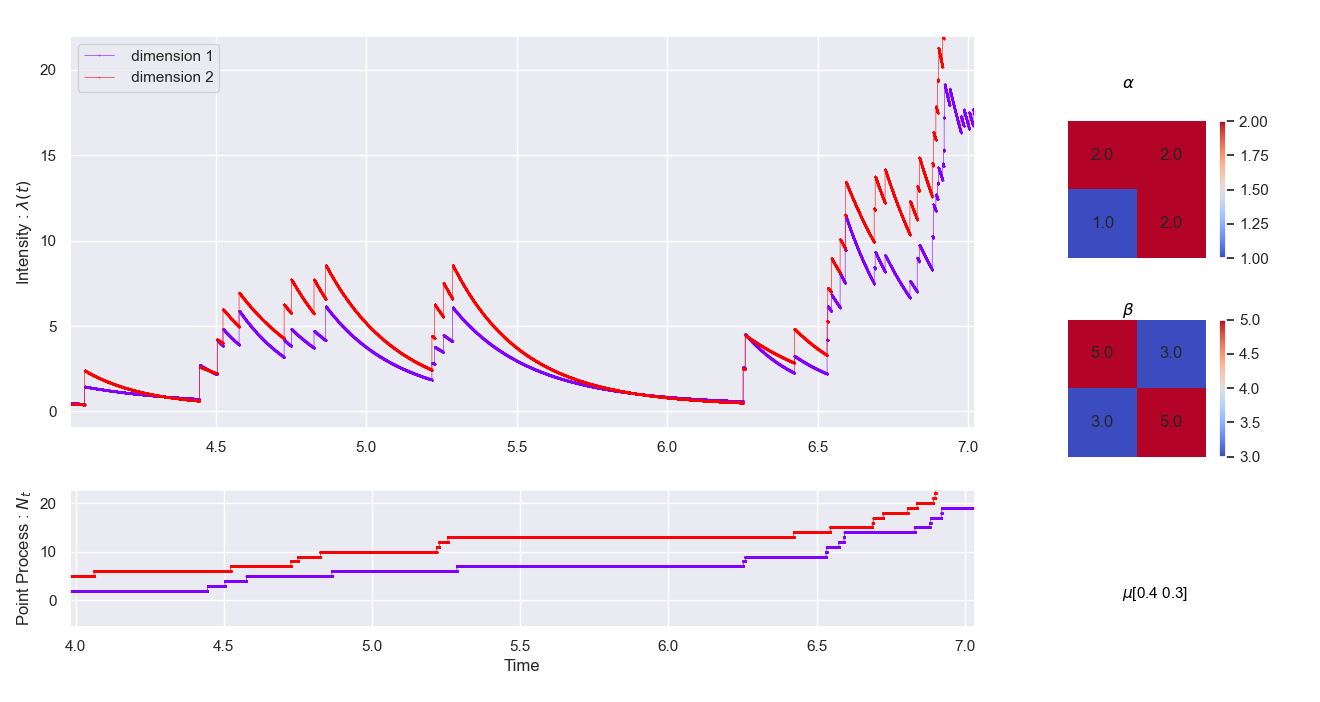
\includegraphics[width = 0.99 \textwidth]{../imag/chap1/hawkes2.png}
\caption{Sampled path from a bivariate Hawkes process. Top: intensity of each process. Bottom: corresponding counting process. The processes $N_t^m$ are shifted for readability. One can notice the interdependence between the two processes. For example, the first jump (from dimension 2) doesn't increase the two processes by the same value. The second jump (from dimension 1) increases the two processes by the same value.}
\label{fig:hawkes2}
\end{figure}


\subsection{Few Remarks about Hawkes Processes}
\begin{remarque}
The process should be considered cadlag. On the other hand, $\lambda^m$ is left-continuous adapted because if the conditional intensity has a discontinuity at some point, then its value should be defined by its history, not by the point itself (cf. \cite{daley}). Since left-continuity of the path implies predictability we use this sufficient condition. 
\end{remarque}

\begin{remarque}
Another interesting kernel is the so-called exponential kernel of order P, that one can define as:

$$ \mu (t) = \sum_{j=1}^P \alpha_j \exp( - \beta_j t ) $$

More details in \cite{exphawkes} and in \cite{exphawkes2}.
\end{remarque}

\begin{remarque}
Another popular choice for the kernel $\mu$ is a power-law function, yielding:

$$ \lambda (t \mid \Tau_{t^-} ) = \nu + \int_{- \infty }^t \frac{ k }{ \left ( c + t - s \right ) ^p } $$

where $c,k,p > 0$. It is widely used in the seismology literature and in the social media literature.
\end{remarque}




\begin{remarque}
The Hawkes process we described is referred to as the linear Hawkes process. Defining the counting process based upon a conditional intensity function of the form:

$$ \lambda (t \mid \Tau_{t^-}) = \Psi \left ( \int_{-\infty}^t \mu(t-s) dN_s \right ) $$ where $\Psi : \R \to \R_+$, we get the so-called nonlinear Hawkes process. \\Setting $\Psi(u) = \nu_1 + u$, the function reduces to the linear case. 

We mention two works related to nonlinear Hawkes processes, that one can discover inside \cite{nonlinearHP1} and \cite{nonlinearHP2}.
\end{remarque}

\begin{remarque}
A last thing about Hawkes processes is the difference between temporal and spatio-temporal Hawkes processes. Spatiality can be incorporated with an additional function convoluting with the kernel. This theoretical domain is pretty useful for seismic studies.
\end{remarque}



\subsection{Self-Regulating Hawkes Process}
\label{section:obral}

The terms 'self-exciting'  (and by opposition 'self-regulating') can be made precise through the conditional intensity function. If an event causes the stochastic conditional intensity function to increase then the process is said to be self-exciting. Empirically, it causes temporal clustering of events. 

On the other hand, if the conditional intensity function is lowered by events, the process is called self-regulating. 

Copying an image from \cite{obral} that one can find at pages $30$ and $31$, that we display on fig. \ref{fig:obral}, we show two graphs representing a self-exciting and self-regulating processes. 

The essential difference if whether the parameters $\alpha$ are taken positive or negative. 

It however changes the model completely (on a philosophical point of view) and could interfere with the estimation process of the parameters, as the boundaries for the algorithms might have to be changed.

Such processes are not examined hereinafter.

\begin{figure}
\centering
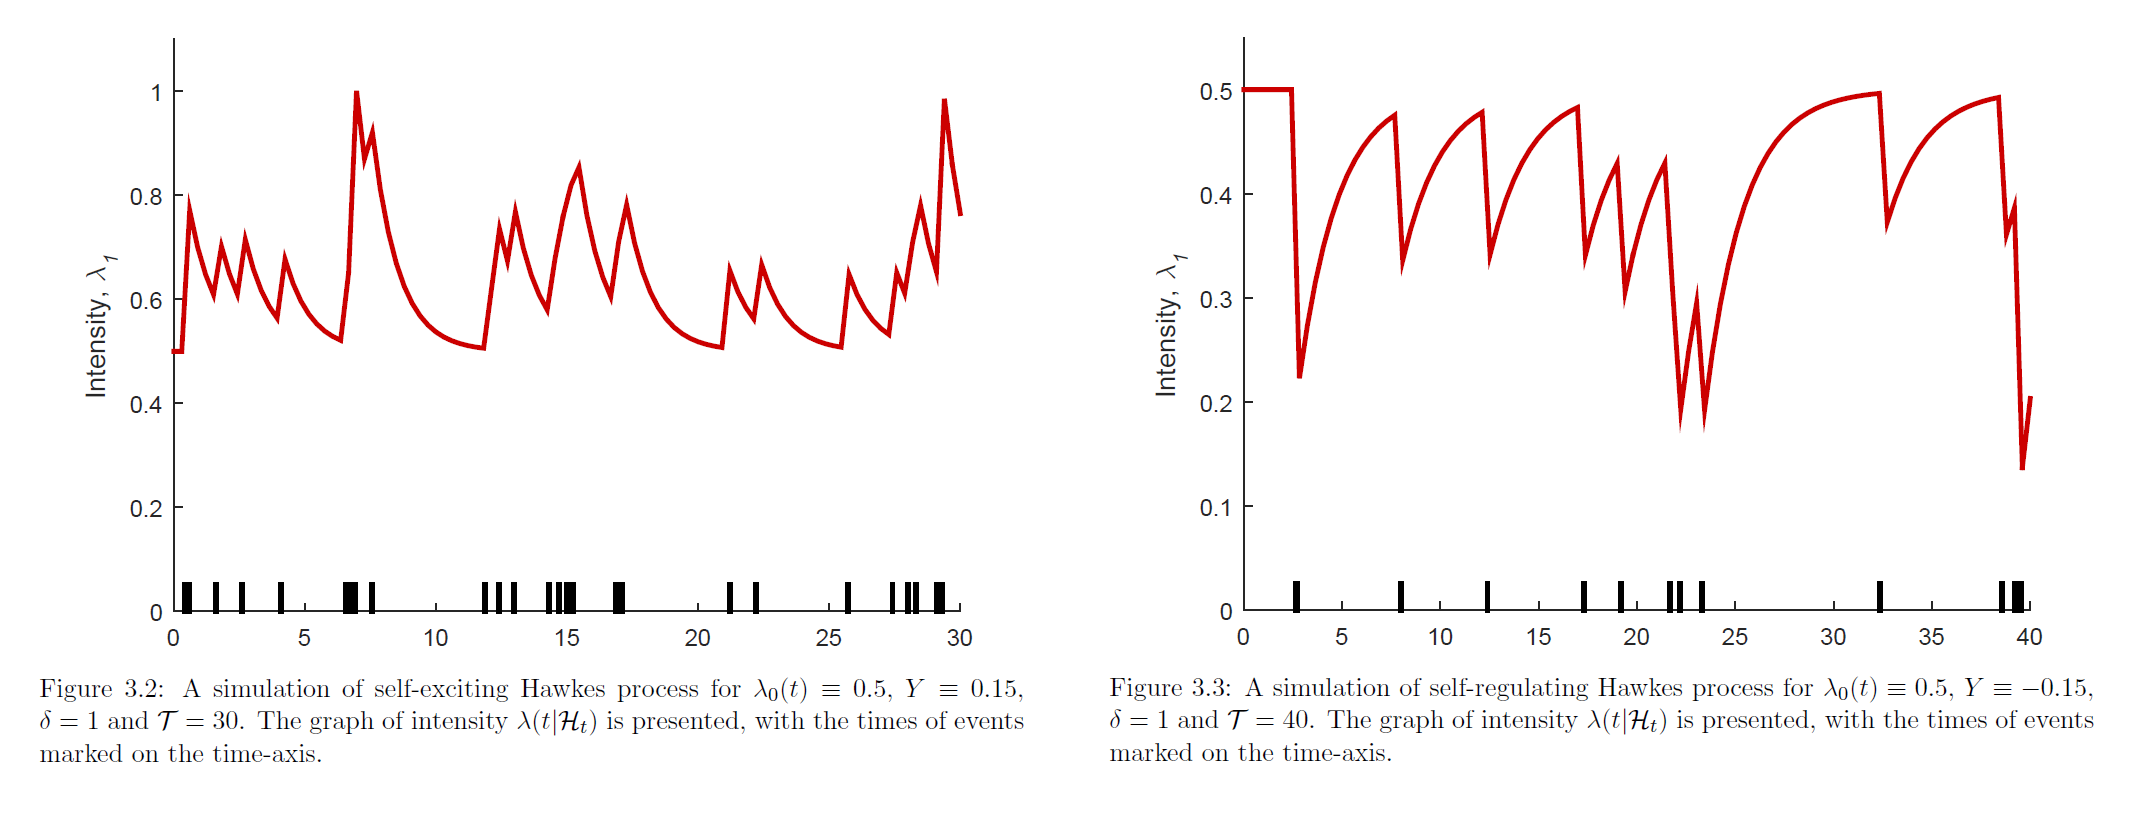
\includegraphics[width = 0.90 \textwidth]{../imag/chap1/obral.png}
\caption{ Plots of self-exciting and self-regulating processes from \cite{obral}.}
\label{fig:obral}
\end{figure}












\subsection{Hawkes Processes as Branching Structures}
We notice that Hawkes process are marked simple point processes.

Another equivalent view is its branching structure, by ignoring the time location of the events. Through the superposition
properties of point processes (cf. \cite{daley}, Theorem 2.4.VI), one can decompose the events into two categories: the immigrants and the offspring. The immigrants are the external events while the offspring is triggered by the previous events in the process. The offspring are structured into clusters associated with the original immigrant parent. That representation is particularly useful for categorizing the different Hawkes process (subcritical / critical / supercritical Hawkes process) as well as for forecast.

Essentially, the immigrants are distributed as a homogeneous Poisson process; the clusters are each associated to one immigrant and all-together form an independent partition of all the immigrants. The number of offspring is given by a Poisson law of parameter equal to the branching factor (defined below). The times of the events can be computed with the inter-arrival times, which in this case (homogeneous Poisson) are exponentially distributed.

An accessible summary about that representation is given in \cite{socialhawkes}. 

\begin{definition}[Branching Factor]
The branching factor is defined as the expected number of direct offspring spawned by a single event. For univariate, un-marked Hawkes process, the branching factor $n^*$ can be computed:

$$ n^* = \norm{ \mu }_{L^1} $$

It is fairly intuitive that when that number is greater than one, the number of immigrants might be infinite. 
\end{definition}


\begin{remarque}
A critical Hawkes process ($n^* = 1$) must not explode, though it usually does. For example, if the kernel is sufficiently long tailed, one can create a stationary Hawkes process without immigration. An example given by Brémaud and Massoulié in 2001 show that when clusters overlap while being far enough, the process might be stationary.
\end{remarque}







\subsection{Marked Hawkes Processes}
\label{subsection:marked}
A natural extension to Hawkes Processes is having stochastic kernels. The simplest example is marked kernels (where the mark is commonly coined $Y$ in the literature), like marked exponential kernels:

$$\mu(t- t_i^j, Y_i^j) =  Y_i^j \exp \left ( - \beta_j \cdot ( t - t_i ) \right ) $$

then the model from eq.(\ref{eq:stieltjes_integral3}) becomes:

\begin{align}
\lambda^m (t \mid \Tau_{t^-} ) &= \nu_m + \sum_{n = 1}^M \sum_{ \{k: t_k^n < t \}} \mu(t- t_k^{n}, Y_k^{m,n}) \notag \\
&=  \nu_m + \sum_{n = 1}^M \sum_{ \{k: t_k^n < t \}}   Y_k^{m,n} e^{- \beta_{m,n} \cdot ( t - t_k^n ) } 
\end{align}

It is a classical practice considering unpredictable marks. 



\subsection{Stability of Hawkes Processes}

\willdo{ How Hawkes is stat. conditions, 1D et multi dim ? est ce que algo fonctionne quand même? }

An interesting question is whether a Hawkes process is stationary. It is a very important question because we want the process to be stable, and to be simulable, which would be easier when the process is stationary.

Following the ideas of \cite{Hawkes}, one can write the conditional intensity process in a matrix form:
\begin{equation}
\overline{\lambda} = \E [ \lambda(t) ] = (I - \Gamma) ^{-1}\overrightarrow{\nu}  
\end{equation}

where $ \Gamma = \norm{\mu}_{L^1} $,  $\mu$ is the chosen kernel for the Hawkes process.
 
In the case of exponential kernels, $\Gamma$ takes a simple form:

\begin{equation}
\forall m,n \in \llbracket 1, M \rrbracket^2: \  \mu_{m,n} (t) = \alpha_{m,n} \exp ( - \beta_{m,n} t ) \implies \Gamma = \left ( \frac{ \alpha_{m,n} } { \beta_{m,n} } \right )_{ m,n \in \llbracket 1, M \rrbracket^2} 
\end{equation}

A sufficient condition for stationarity of the process is the spectral radius of $\Gamma$ is strictly less than 1. This is due to the fact that since the immigrant process is stationary, all we need is that the mean cluster size to be finite. Recall that the spectral radius of the matrix $\Gamma$ is defined as the maximal value of the set of the absolute eigenvalues of $\Gamma$.

In the case of marked Hawkes processes, the matrix $\Gamma$ has a slightly different form. We follow the computations from \cite{my_algo_simul}.

\willdo{ici !!! à écrire; suivre 22.}


\section{Simulation for Fixed Parameters}
\subsection{Notations}

The author refers to paper \cite{my_algo_simul} for an interesting solution in order to simulate Hawkes processes. There are different easier ways to simulate a Hawkes process (cf. appendix \ref{appendix_simulate}). However, they do not give as much flexibility as the one from \cite{my_algo_simul} and that's the reason why we use it. It is in fact, even more general than what we need. The algorithm allows the simulation of Marked Multidimensional Hawkes processes. We focus on marks being deterministic (thus we can assume that the parameters are constant).


The algorithm is the following. It is based on the idea that one can simulate the waiting time between jumps. For a $M$-dimensional process, each dimension has an impact on the other. Hence, we can simulate the waiting time for every dimension influencing every other dimension (including itself).




\begin{itemize}
\item $r_j$ is the time of the $j$-th jump and $r_0$ is by convention $0$. We define the vector $\overrightarrow{r} = \sequence{r_i}$ as being the sorted times for all events in the Hawkes processes. 
\item we also define $\overrightarrow{t}^m = \sequence{ t_i^m } $ as being the jumps' time for one marginal process. Clearly, there is the following relationship between $\overrightarrow{r}$ and $\overrightarrow{t}^m $:
$$ r = \bigcup_m \bigcup_k  t_k^m $$
\item $a_{m,j}^i$ reads the waiting time after jump $(j-1)$-th and the jump created by process $i$ upon process $m$ (thus corresponding to intensity $ \lambda^i_m$). In other words, the $i$ index indicates which dimension is triggering the jump, the $m$ index corresponds to the dimension which receives the jumps. This decomposition of the intensity is the rational of the followability of the algorithm, as defined in section \ref{section:definition_algo}.


\begin{remarque}
$$\forall m,j \in  \llbracket 1, M \rrbracket, \qquad a_{m,j}^i \sim \mathcal L_{m,j}^i   $$
Where $\mathcal L_{m,j}^i $ is defined by the CDF:
\begin{align}
F(s) &= 1 - \exp \left ( - \int_{r_{j-1}}^{r_{j-1} + s } \lambda_m^i (t) dt \right ) \notag \\
&= 1 - \exp \left ( - \frac { \lambda^i_m ( r_{j-1} ) } { \beta_m^i } ( 1 - e^{ - \beta_m^i s} ) \right )
\label{eq:L_defined}
\end{align}

Hence, we can use the inverse CDF method. It consists in inverting the previous CDF and generating a uniform random variable. The process is described in algorithm \ref{algo:CDF_1}.
\end{remarque}



\begin{algorithm}[H]
\label{algo:CDF_1}
\SetAlgoLined
$u \sim U(0,1)$,

\eIf{ $u < 1 - \exp \left ( - \frac { \lambda^i_m ( r_{j-1} ) } { \beta_m^i } \right ) $ }{
we let 
\begin{equation}
a_{m,j}^i = - \frac{1} { \beta_m^i} \ln \left ( 1 + \frac{ \beta_m^i } { \lambda^i_m ( r_{j+1} ) } \ln ( 1 - u ) \right )
\label{eq:cdf_invert}
\end{equation}
}
{$ a ^i_{m,j} = \infty $.}
\caption{Generate the waiting time of the self-exciting part.}
\end{algorithm}


Notice that there is a typo in the original document. The good formula is the one written above\footnote{One can compare the previous line (eq. \ref{eq:cdf_invert}) with the equation (20) from \cite{my_algo_simul}.}.

Also notice that the CDF defines a defective random variable ( as defined in \cite{my_algo_simul}). It means the random variable has a probability mass at $\infty$. Indeed:

$$ \mathbb P ( a^i_{m,j} = \infty ) = \exp \left ( - \frac { \lambda^i_m ( r_{j-1} ) } { \beta_m^i } \right ) > 0 $$



\item $a_{m,j}^0$ is the waiting time for the natural immigration process upon process $m$, meaning the process without the self-excitement part. 

\begin{remarque}
In order to sample $a^0_{m,j}$,
$$\forall m,j \in  \llbracket 1, M \rrbracket, \qquad a_{m,j}^0 \sim \exp( \nu_m )$$
Hence, we can use the inverse CDF method. 
\end{remarque}

\item $N^{m} (t) $ the counting process, underlying the marginal $m$-th Hawkes process, at time $t$.
\end{itemize}


Finally, one should know that the update rule for the intensity cache is given as follows, where:

\begin{equation}
\lambda_m^i ( r_j ) = \lambda_m^i ( r_{j-1} )  e^{ - \beta_m^i \min_{m,i} a_{m,j}^i } + \alpha_{i,m} \11charac_{i = m^*}
\label{eq:update_lambda} 
\end{equation}

Notice that by adjusting this expression, one can easily get the plot of the intensity of a Hawkes process:

\begin{equation}
\label{eq:update_lambda_plot} 
\forall t \in ]r_{j-1}, r_j ], \quad \lambda (t)_m^i = \lambda_m^i ( r_{j-1} )  e^{ - \beta_m^i ( t - r_{j-1} }
\end{equation} 

where we excluded the left bound because the process is left continuous.
 
With all those notations, we are ready to introduce the algorithm \ref{algo:simul_hp} in the following section.









\subsection{Algorithm for Fixed Parameters}



\begin{algorithm}[H]
\label{algo:simul_hp}
\SetAlgoLined

\For{ $j > 0$ }
			{ \While {$r_j < T$}
					{\For{$m \in \llbracket 1, M \rrbracket$}
						{Sample $a_{m,j}^0 \sim \exp( \nu_m ) $,
						
						\For{$i \in \llbracket 1, M \rrbracket$}
							{Sample $a_{m,j}^i \sim  \mathcal L^i_{m,j} $, as defined by \ref{eq:L_defined},
							}
						}
						
						$r_j = r_{j-1} + \min_{m,i} a_{m,j}^i$,
						
						\For{$m \in \llbracket 1, M \rrbracket$}
							{Update $\lambda_m^i ( r_j )$ according to equation (\ref{eq:update_lambda}),
							
							Update $N^m ( r_j ) = N^m( r_{j-1} ) + {\11charac}_{m = m^*} $,}
					$t_k^{m^*} = r_j$ where $k = N^{m^*} ( r_j ) $ and $ m^*,i^* = \argmin_{i,m} a_{m,j}^i $,
					}
			Discard the last $r_j$ > T.
			}
\caption{Exact simulation of multidimensional Hawkes process}
\end{algorithm}



\begin{remarque}
As illustration, $i^* = 0$ then $r_j$ is an immigrant; $m^* = i^*$ implies that the jump arises from self-excitation; otherwise, $r_j$ is caused by an external process $i^*$.
\end{remarque}

\begin{remarque}
Notice that the algorithm also works for $\alpha_{m,n} < 0$. One should however be cautious of not having a strictly negative intensity. Also, $\alpha_{m,n}$ can be potentially replaced by a random variable transforming the point process into a marked point process (more details in the original paper \cite{my_algo_simul}).
\end{remarque}

We can observe a sample path for a uni-variate and penta-variate Hawkes process in the following figures: \ref{fig:hawkes1} and \ref{fig:hawkes5}.

\begin{figure}
\centering
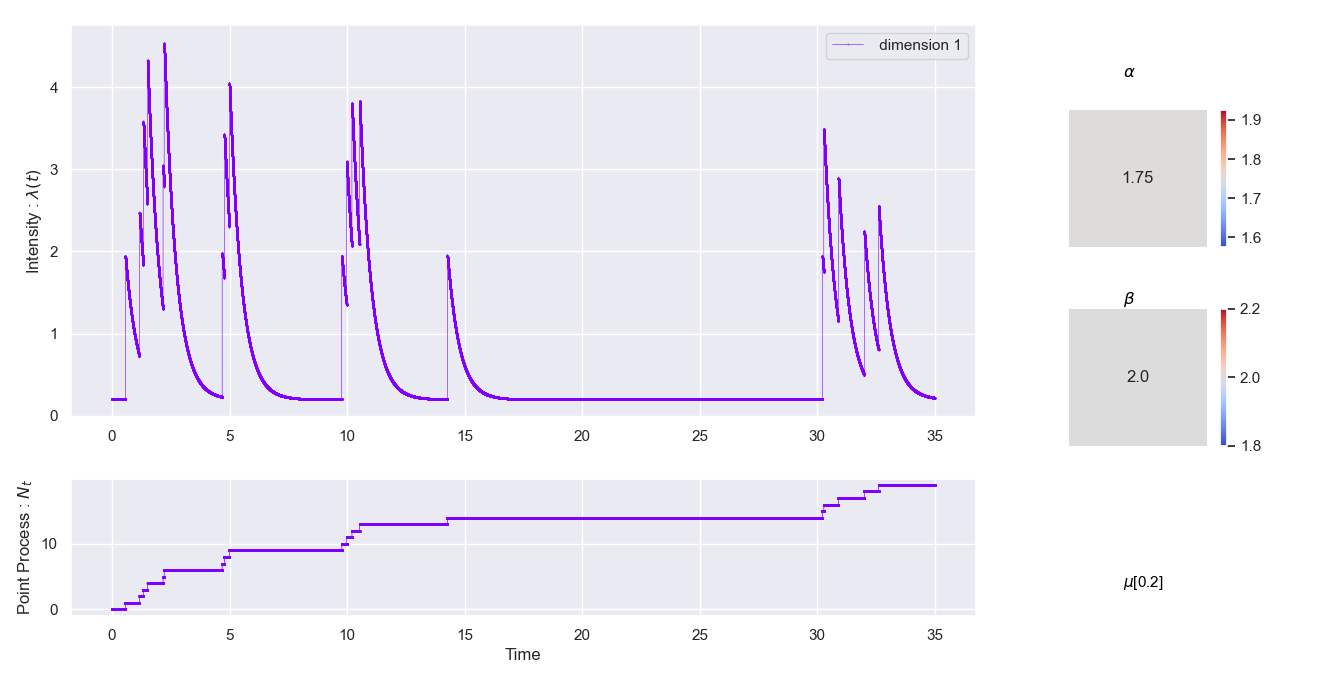
\includegraphics[width = 0.99 \textwidth]{../imag/chap1/hawkes1.png}
\caption{Sampled path from a uni-variate Hawkes process. One can easily distinguish the clusters.}
\label{fig:hawkes1}
\end{figure}


\begin{figure}
\centering
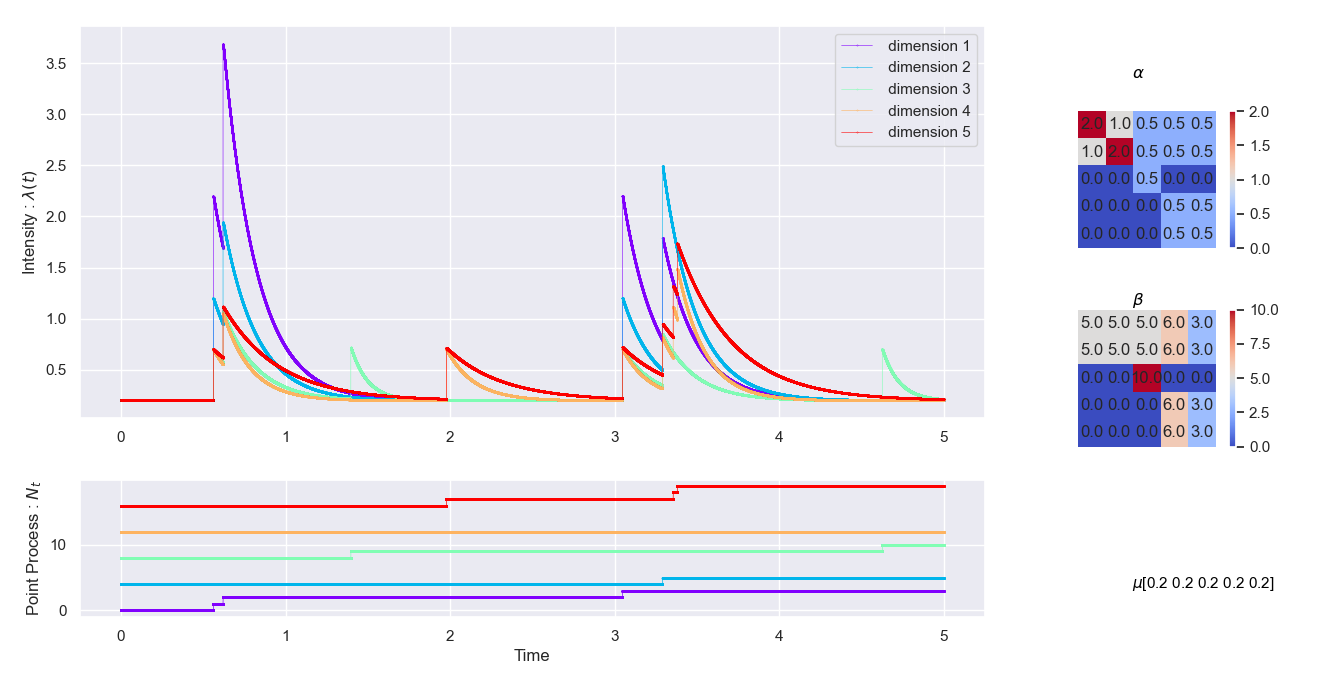
\includegraphics[width = 0.99 \textwidth]{../imag/chap1/hawkes5.png}
\caption{Sampled path from a penta-variate Hawkes process. Top: intensity of each process. Bottom: corresponding counting process. The processes $N_t^m$ are shifted for readability.}
\label{fig:hawkes5}
\end{figure}

\subsection{Edge Effect}
\label{subsection:edge}
Edge effect is defined in \cite{socialhawkes} in the following manner:

\textit{In practical applications, the process might have started sometime in the past, prior to the moment when we start observing it, denoted as $t = 0$. Hence, there may be unobserved event times which occurred before time $0$, which could have generated offspring events during the interval $[0;T]$. It is possible that the unobserved event times could have had an impact during the observation period, i.e. sometime after $t > 0$, but because we are not aware of them, their contribution to the event intensity is not recorded.}


Some interesting discussions can be found in \cite{daley}, as well as in these two papers that directly refer to edge effect: \cite{cox}, \cite{rasmussen}. The proposed methods could potentially be added to any other algorithm summarized in table \ref{table:methods_HP}.



\willprecise{understand if it is the same thing as burn in and talk about it}

\section{Simulation for Time-Dependent Parameters}
\subsection{Preliminary}

The algorithm from \cite{my_algo_simul} allows to simulate multidimensional Hawkes processes, with different decays parameters, for an exponential kernels with marks, and constant immigration rates. From that, it is obvious that one can use the previous algorithm with deterministic jumps ($\alpha$). On the other hand, the underlying intensity ($\nu$) is easily changeable by using any method for simulation non-homogeneous Poisson process.

However, the task is way harder concerning the decays ($\beta$).

To sum-up:
\begin{itemize}
\item deterministic $\alpha$ is already included in the previous algorithm.
\item deterministic $\beta$??????  The task with beta is quite harder. A usual choice is a parameter piecewise constant. 
\item deterministic $\nu$ needs some work. We are using a basic and classical thinning algorithm for that. One can find more about it in appendix part \ref{subsection:thinning}.
\end{itemize}




\willprecise{talk about the betas it with Ed}

It would also be possible to compute the CDF of the interarrival times related to a function $\nu(t)$ and inverse the formula. However, such approach makes it compulsory to solve equations by hand in order to find the inverse. The inverse can be more or less challenging to find. 


\begin{theoreme}{Non-homogeneous Poisson process interarrival times}
If the process has intensity $\nu(t)$, one gets that the pdf of the $n$-th jump's time is 

$$
f_n(t)  = \frac {\left ( \int_0^t \nu(s) ds \right )^{n-1}}{(n-1)!} \nu(t) e^{-  \int_0^t \nu(s) ds }
$$

Then the CDF for the $n$-th jump's time is:

$$
F_1(t) = 1 - e^{  \int_0^t \nu(s) ds } 
$$

\end{theoreme}

\willdo{finish the proof}

\begin{demo}{}{}
First recall that by definition of Poisson process with rate $\lambda$, one has:
$$
\mathbb P(N_t = k) = \frac { (\lambda t)^k \exp(- \lambda t ) }{k !}$$

Non-homogeneous Poisson process can be seen as a homogeneous Poisson process with a non-constant intensity function $\lambda (t)$. It can be proven (cf. \cite{Veraart}), that we also have the previous formula for non-homogeneous Poisson processes, meaning:

$$
\mathbb P(N_t = k) = \frac { \left ( \int_0^t \lambda(s) ds \right )^k \exp \left ( - \int_0^t \lambda(s) ds \right )  }{k !}$$

then from \begin{verbatim}
https://www.randomservices.org/random/poisson/
Nonhomogeneous.html
\end{verbatim}

Using the identity from theorem \ref{thrm:point_counting}.

$$ P( N_t \geq n ) = \sum_n^{\infty} \exp \left ( - \int_0^t \nu(s) ds \right ) \frac{ \left ( \int_0^t \nu(s) ds \right ) ^k }{k !} 
$$
\end{demo}


\begin{ajoutationV}{}{}
If one searches the inverse of a function of the following form:

$$ y(x) = 1 - \exp ( - (\alpha x + \beta x^2) ) $$

we get:

$$ x(y) = \frac{- \alpha \pm \sqrt{\alpha^2 - 4 \beta \ln(1-y) }  }{2 \beta}$$

Whenever $r_j$ is the time location of the jump, $s$ the time-location after $r_j$ when the next jump occurs. Replacing $$\alpha s + \beta s^2 = ( b + a r_j ) s + \frac 1 2 a s^2 $$ 
we get back to the scenario $$ \nu(t) =  a t + b $$ which is one of the four models we considered in fig. \ref{fig:evol_functions}.
\end{ajoutationV}


\subsection{Algorithm for Time-Dependent Parameters}

In order to simulate the underlying non-homogeneous Poisson process, we define the following law:
$$ \forall m,j \in  \llbracket 1, M \rrbracket, \qquad a_{m,j}^0 \sim \mathcal J_m  $$

Where $\mathcal J_m $ is defined by the CDF:
\begin{equation}
\label{eq:J_defined}
F(s) = 1 - \exp \left ( - \int_{r_{j-1}}^{r_{j-1} + s } \nu_m (t) dt \right )
\end{equation}

We also need the following equation, which deals with the deterministic $\alpha$\footnote{The only difference is that now we consider $\alpha$ as a function of the time.}:

\begin{equation}
\lambda_m^i ( r_j ) = \lambda_m^i ( r_{j-1} )  e^{ - \beta_m^i \min_{m,i} a_{m,j}^i } + \alpha_{i,m} (r_j) \11charac_{i = m^*}
\label{eq:update_lambda_time} 
\end{equation}




\begin{algorithm}[H]
\label{algo:simul_hp_time}
\SetAlgoLined

\For{ $j > 0$ }
			{ \While {$r_j < T$}
					{\For{$m \in \llbracket 1, M \rrbracket$}
						{Sample $a_{m,j}^0 \sim \mathcal J_{m} $ as defined by \ref{eq:J_defined} using a thinning algorithm (cf. algorithm \ref{algo:thinning_algo} in appendix),
						
						\For{$i \in \llbracket 1, M \rrbracket$}
							{Sample $a_{m,j}^i \sim  \mathcal L^i_{m,j} $, as defined by \ref{eq:L_defined},
							}
						}
						
						$r_j = r_{j-1} + \min_{m,i} a_{m,j}^i$,
						
						\For{$m \in \llbracket 1, M \rrbracket$}
							{Update $\lambda_m^i ( r_j )$ according to equation (\ref{eq:update_lambda_time}),
							
							Update $N^m ( r_j ) = N^m( r_{j-1} ) + {\11charac}_{m = m^*} $,}
					$t_k^{m^*} = r_j$ where $k = N^{m^*} ( r_j ) $ and $ m^*,i^* = \argmin_{i,m} a_{m,j}^i $,
					}
			Discard the last $r_j$ > T.
			}
\caption{Exact simulation of multidimensional Hawkes process}
\end{algorithm}


\vspace{0.5cm}

One can see a few example of realized univariate processes where the parameters change over time in fig. \ref{fig:param_dep_hawkes}. 


\begin{figure}
\centering
\subfloat{{
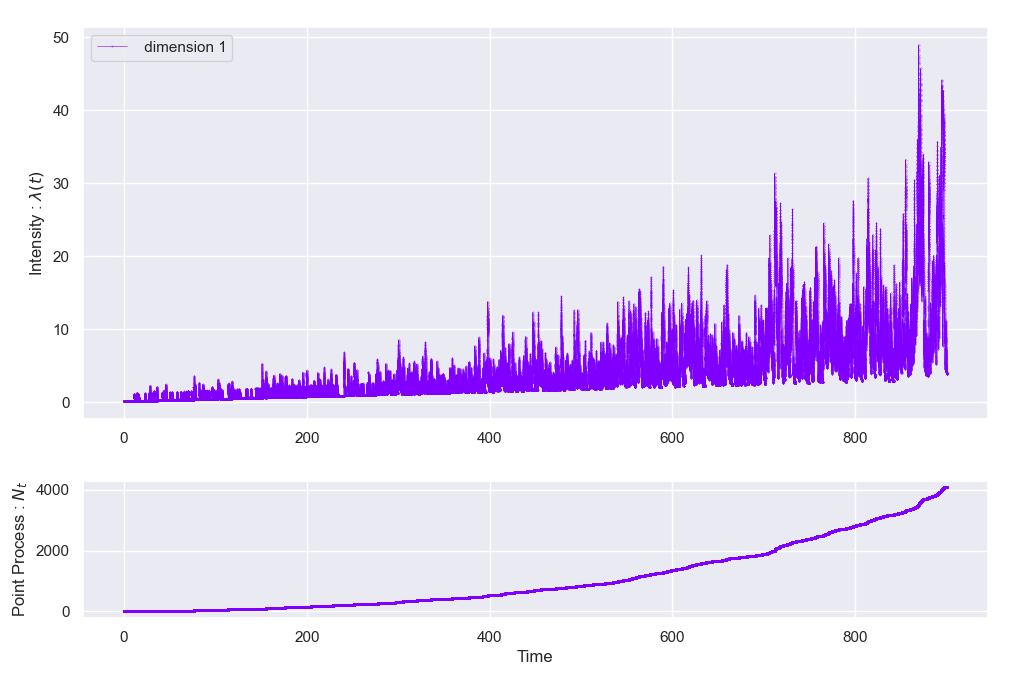
\includegraphics[width = 0.48 \textwidth]{imag/chap2/simul/Hawkes_linear.png}
}} 
\subfloat{{
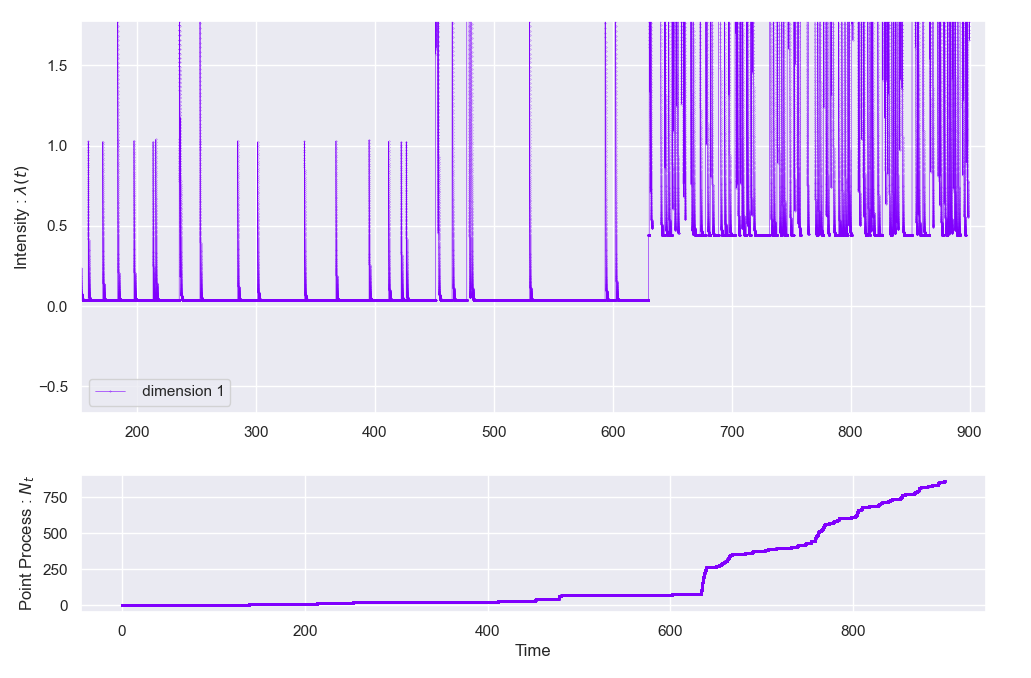
\includegraphics[width = 0.48 \textwidth]{imag/chap2/simul/Hawkes_jump.png}
}}\\
\subfloat{{
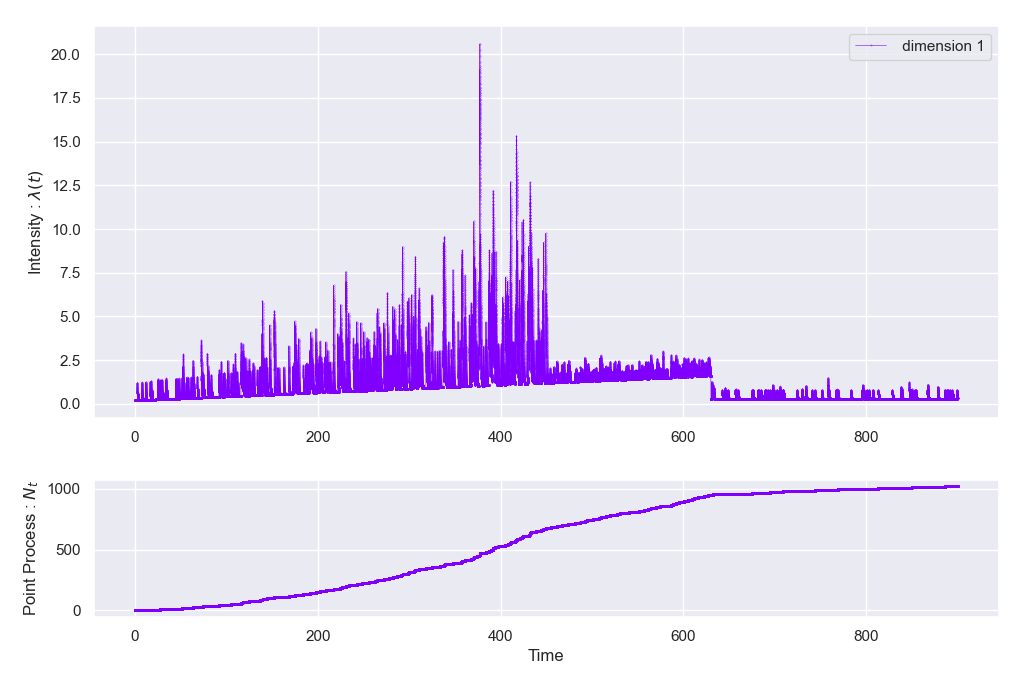
\includegraphics[width = 0.48 \textwidth]{imag/chap2/simul/Hawkes_mountain.png}
}} 
\subfloat{{
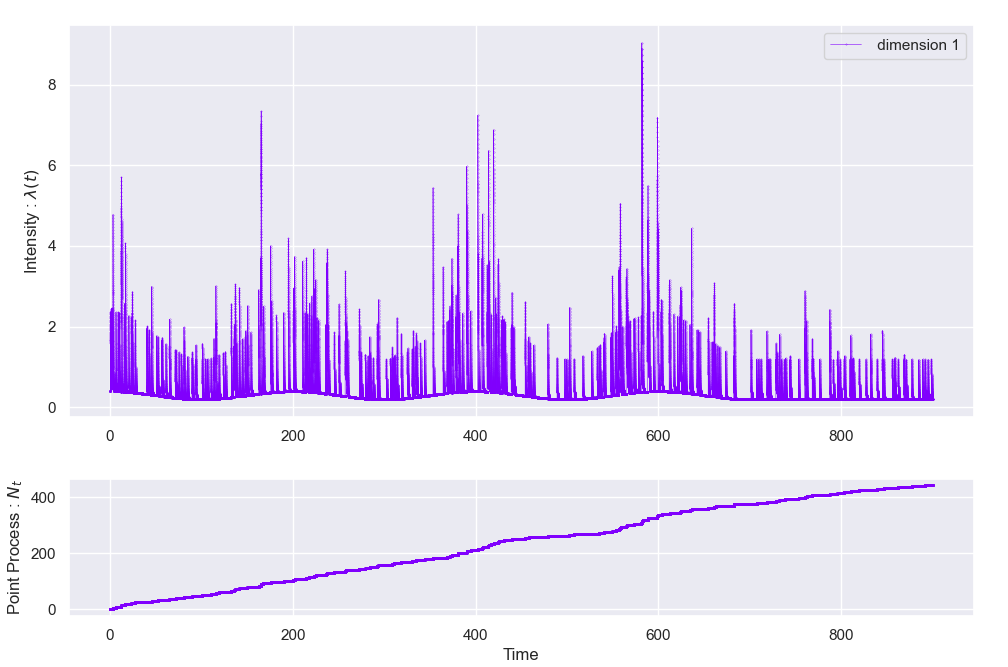
\includegraphics[width = 0.48 \textwidth]{imag/chap2/simul/Hawkes_sin.png}
}}

\caption{On the basis of the functions from fig. \ref{fig:evol_functions}, we modify $\alpha$ and $\nu$ with respect to time. One can notice the jumps, as well as the underlying intensity, changing with respect to time. For the one corresponding to "one jump" function, we zoomed in in order to emphasize the phenomena.}
\label{fig:param_dep_hawkes}
\end{figure}











\section{Our Numerical Solution}
\willdo{ talk about code?}
\subsection{Classes}
\subsection{Functions}



